\documentclass[prl,twocolumn,superscriptaddress,floatfix]{revtex4}
\usepackage[utf8]{inputenc}
\usepackage{graphicx}
\usepackage{float}
\usepackage{amsmath,amssymb,amstext}

% get rid of hbox badness 10000 in bbl file
\usepackage{etoolbox}
\apptocmd{\sloppy}{\hbadness 10000\relax}{}{}

% graphicspath to images dir
\graphicspath{{./images/}}

\begin{document}

\title{Measurement of Resistivity at Low Temperatures}
\author{Robbie Ellis, Junseo Shin, and Daniel Rothstein}
\affiliation{Department of Physics, Washington University, St.\ Louis, Missouri 63130}

\date{\today}

\begin{abstract}
    At low temperatures, materials can experience phenomena such as superconductivity and magnetic ordering. For Lead (Pb) and Niobium Titanium (NbTi), there is a critical temperature $T_C$ where the characteristics of superconductivity appears \cite{1062311}\cite{PhysRev.109.1094}.
    %When the temperature of Dysprosium (Dy) goes below its Curie Temperature, it undergoes ferromagnetic ordering which changes the crystal structure of the material to align spins and become magnetic. %I commented this out because we didnt talk about it later
    For Copper, at low temperatures, the phonon contribution to the resistivity changes from a $T$ scaling to a $T^5$ scaling, which can be described by the Bloch-Gr\"uneisen formula \cite{ZimanEP}. Dysprosium is also known to transition from a paramagnetic state to a ferromagnetic state below 179 K, further highlighting the diversity of low-temperature behaviors in
    materials \cite{Wilkinson1961-mk}.
    %In addition to the challenges imposed by the lab equipment and apparatus for low temperature experiments,
    %the techniques and protocols followed to measure materials at certain temperatures are crucial to the precision and accuracy of data acquisition.
    In this experiment, the temperature and resistivity of these materials are measured at low temperatures to re-evaluate the known properties of these materials described in the literature. %no what
    %The results from this experiment show systematic errors due to the limitations of the equipment and tools used in lab.
    %with the correct intuition and understanding of the how these error propagate through the data.
    Despite equipment limitations and fragmented data collection, examination of the recorded data displays the mentioned phenomena very clearly, which
    provides critical information to understand the properties of materials at low temperatures.
\end{abstract}
\maketitle

% cite with \cite{key}
% quote with ``quote''

% Suggestion for maintaining figures:
%   separate dir for figures/images 
%   use \graphicspath{{../images/}} in preamble

% e.g. simple figure
% \begin{figure}[H]
%     \begin{center}
%     \includegraphics[width = 0.3\textwidth]{filename.pdf}
%     \caption{[CAPTION HERE]}
%     \label{fig:number}
%     \end{center}
% \end{figure}
% refer to figure with Fig. \ref{fig:number}

% possible double (vertical)
% \begin{figure}[H]
%     \begin{center}
%     \includegraphics[width = 0.3\textwidth]{filename1.pdf} (add & for side by side)
%     \includegraphics[width = 0.3\textwidth]{filename2.pdf}
%     \caption{\label{fig:number}[CAPTION HERE] (add & for side by side)}
%     \end{center}
% \end{figure}

% e.g. simple table
% \begin{table}[H]
%     \begin{center}
%     \begin{tabular}{|c|c|}
%     \hline
%     [HEADER 1] & [HEADER 2] \\
%     \hline
%     [DATA 1] & [DATA 2] \\
%     \hline
%     \end{tabular}
%     \caption{[CAPTION HERE]}
%     \label{tab:number}
%     \end{center}
% \end{table}
% refer to table with Table \ref{tab:number}

\section{Introduction}
In 1911, Dutch physicist Heike Onnes discovered a sudden disappearance of electrical resistance in solid Hg at a temperature of $4.2\text{K}$ with the use of liquid helium as a cooling agent \cite{Van_Delft2010-ra}. This low resistance state, now referred to as a ``superconducting" state, has been observed in several other materials, such as Pb, NbTi, and several other metals/metalic compounds. Around 20 years after Onnes' discovery, two German physicists, Walther Meissner and Robert Ochsenfeld discovered that a material in a superconducting state will prevent the formation of an internal magnetic field in the presence of an external magnetic field. This phenomenon, known as the Meissner effect, arises from the generation of surface currents which contribute a magnetic field essentially equal in magnitude and opposite in direction of the induced internal field \cite{Kittle}. These discoveries uncovered a few of the interesting and unpredictable ways in which matter behaves at low temperatures.

When considering properties of solids, it is necessary to consider how the lattice of nuclei interact with electrons in the material. While there are obvious Coulomb forces, there are also other interactions that electrons participate in. Vibrations in lattice elements will arise as a result of nuclei being moved slightly from equilibrium–this vibration is quantized, with quanta known as phonons. While these phonons are not real particles (unlike a photon, which would analogously be thought of as a quanta of a “vibration” in the electromagnetic field), they share many similar properties. For example, phonons couple to electrons as an actual particle (such as a photon) would. An important aspect of phonons is that they obey Bose-Einstein statistics, and are not conserved–this results in an equilibrium distribution analogous to that of photons:
\begin{equation}
f(E,T)=\frac{1}{e^{\frac{E}{T} }-1}
\end{equation}
considered in natural units, with $k=\hbar=c=1$. 

The more interesting aspects of phonons arise from the fact that there is a minimum wavelength, which can be seen to be twice the distance between adjacent points in the lattice ($L$). This minimum wavelength puts an upper bound on the possible energies a phonon can have, since $E =\frac{c_{s}}{2\pi \lambda}$ (where $c_s$ is the speed of sound in the material), which can be seen as a generalization of the equation for photon energy (given in natural units). In materials where the distance between lattice points is the same in all dimensions, it is evident that the possible energy states are confined to a cube, with side lengths proportional to $\frac{1}{L}$. This cutoff makes the properties of the phonon population greatly temperature dependent, resulting in a number density proportional to $T^{3}$ at low temperatures, and $T$ at high temperatures \cite{Kittle}.

It can also be shown that at low temperatures, the number of scattering events that contribute to the resistivity of the material scales as $T^2$, while at higher temperatures phonons will have enough energy on average to make every collision contribute to resistivity–therefore, the phonon contribution to resistivity is predicted to be proportional to $T^5$ at lower temperatures, and $T$ at higher temperatures \cite{Kittle}.

These principles can be used to form a quantitative model for resistivity due to electron-phonon interactions, which is encapsulated by the Bloch–Gr\"uneisen formula
\begin{equation}
\rho(T)=\rho_{0}+4\rho_{\Theta}\left(\frac{T}{\Theta}\right)^{5} \int_{0}^{\frac{\Theta}{T}} \frac{u^{5}}{(e^{u}-1)(1-e^{-u})}\text{d}u
\label{bloch-gruneisen}
\end{equation}

where $\Theta$, the Debye temperature, determines the temperature at which the transition from $T^5$ and $T$ resistivity scaling occurs, and is given by $\frac{c_s}{4\pi}(\frac{6N}{\pi V})^{\frac{1}{3}}$, where $N$ is the number of atoms in the material and $V$ is it’s volume \cite{ZimanEP}. $\rho_{\Theta}$ is a material-specific constant which describes the strength of the electron phonon coupling, and $\rho_{0}$, the residual resistivity, is the resistivity present at around $0$ K. $\rho_{0}$ can also be used to calculate the materials residual resistivity ratio (RRR), a useful material constant describing the ratio of resistivities measured at 293 K and 4.2 K. In most materials, the resistivity will be approximately constant below $4.2$ K, in which case $\rho_0$ to be used for the materials resistivity at 4.2 K. In materials that superconduct, a RRR value cannot be assigned in the same way as a result of the resistivity dropping to 0 $\Omega \cdot$m. Instead, the resistivity just before the transition to superconductivity is used in place of $\rho_{0}$.

Some models of superconductivity (namely, the Bardeen-Cooper-Schrieffer theory) also attribute the phenomenon to electron-phonon coupling. At low enough temperatures, slight attraction between electrons due to electron-phonon coupling can result in the electrons forming a paired state (called a ``Cooper pair''), which follows Bose-Einstein statistics. As a result, other electrons can form the same state, which results in a perfectly coherent state of Cooper pairs that are stable against disturbances that would normally cause resistivity, resulting in a current that experiences zero resistivity.

Another interesting phenomenon that occurs at lower temperatures is magnetic ordering–once the temperature falls below a certain threshold, materials that are paramagnetic at higher temperatures can undergo a phase transition and become ferromagnetic (or antiferromagnetic). In this state, electrons in the material stabilize themselves by aligning their spins to match (to be opposite of) their neighbors. This phase transition results in a noticeable, abrupt change in the resistivity of the material.

This experiment will highlight these phenomena in various materials. The voltages across samples of Pb and NbTi will be measured to infer resistivity, allowing the superconductivity transition temperature to be measured. The same process will also be applied to Cu and Dy to calculate its Debye temperature and RRR, and the temperature of magnetic ordering, respectively.

    % Superconductivity was first observed in 1911 by Heike Onnes when studying mercury. He found at about 4.2K resistance went to near zero, a superconducting state. Since his experiment, this state has been found in many materials, such as lead and niobidum-titanium. An additional effect of superconductor was found 20 years later by Walther Meissner and Robert Ochsenfeld. They observed a superconductor would not let any magnetic field in. A metal can not superconduct if the temperature is too high or the external magnetic field is too large.
    % However, while some metals superconduct, they do not always do it in the same way.
    % When heating up and applying a magnetic field to type I superconductors, like NbTi, they will suddenly jump to having a higher resistance, and then they will have a linear relationship between resistance and temperature that is normally seen at high temperatures. 
    % Meanwhile, for type II superconductors, like Pb, when they reach the critical point instead of immediately jumping, resistance will rapidly rise with more and more external field and temperature until a second critical point where it returns to linear behavior. This is because type two superconductors experience parts that have higher resistance called vortexes from the circle of current separating the two sections. 
    % Some metals, however, do not experience superconductor. In solid metal latices, the bonds between different atoms can be viewed a spring, keeping the atoms close but not too close. When there is a disturbance to this latices 

    

\subsection{Methodology and Setup}

% replace with better one

\paragraph{Low Voltage Measurements}
In order to measure voltage across the samples effectively we used four-terminal sensing.
In four-terminal sensing, separate pairs of wires handle the current supply and voltage measurement functions,
which minimizes the resistances of the lead wires.

\begin{figure}[ht]
    \begin{center}
    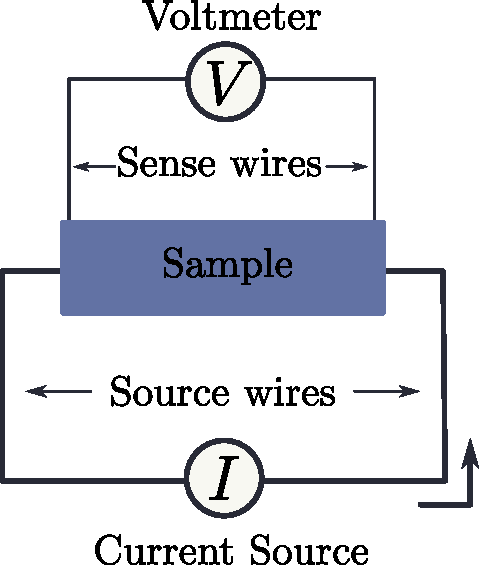
\includegraphics[width = 0.3\textwidth]{4terma.pdf}
    \caption{A diagram of a four terminal sensing apparatus}
    \label{fig:4term}
    \end{center}
\end{figure}

The two ``source" wires supply a current $I$ across the samples,
while the two ``sense'' wires measure the voltage drop $V$ directly across the sample without any additional voltage drop from the wires carrying current, as seen in Figure \ref{fig:4term}.
This ensures that the measured voltage reflects only the drop over the sample itself instead of in the lead wires.
The 4-wire sensing method is a fundamental procedure used to measure voltages for low temperature materials which is 
then used to measure the temperature and resistivity of the sample.

Using the sensitive voltage measurements across the sample,  the resistivity can be determined by first
calculating the resistance across each sample using Ohm's Law, $R = \frac{V}{I}$. 
Then the resistivity of a sample can be calculated using the formula \begin{equation}
\rho = R\frac{A}{L}
\label{eq:resistivity}
\end{equation}
where $A$ is the cross-sectional area of the sample and $L$ is the length of the sample---i.e.
Cu and NbTi wires have a circular cross sectional area $A = \pi r^2$ while Dy and Pb are thin foils with area $A = w \cdot t$. The values for current through these materials were 1 mA for Cu and NbTi, and 30 mA for Dy and Pb.

In order to measure the temperature of each sample, there is a similar resistor with a fixed relationship between resistance and temperature. Using Ohm's law, $V=IR$ , the resistance can be found which has a known relationship to temperature. Then a Chebyshev polynomial (with coefficients provided by the Cernox manufacturer's manual) was used, which relates the log resistance to the log temperature \cite{manuel},
\begin{equation}
%\begin{align*}
    \log_{10} T = \sum_{i} a_i \cos(iw \log_{10} R) + b_i \sin(iw \log_{10} R)
%\end{align*}
\label{calibrate}
\end{equation}
In addition, the Cernox thermometer recommends excitation currents of $100$ $\mu$A for above 30 K,
$10$ $\mu$A for $30 \to 2.5$ K,
and $1$ $\mu$A for below 2.5 K to prevent the internal heating of the thermometer from affecting the temperature measurements.

To minimize heat transfer between the sample and the environment, the samples is housed in two dewars (double walled container):
the inner dewar contains the sample and liquid helium (LHe) being sealed by a variable vacuum, while the outer dewar has an open top which is filled with liquid nitrogen and surrounded by a permanent vacuum jacket.
Furthermore, there are three vacuum pumping systems in place to precisely control the pressures of the inner vessel containing the sample and the variable vacuum as the sample is cooled to low temperatures. 

\paragraph{Low Temperature Procedure}

\begin{figure}[ht]
    \begin{center}
    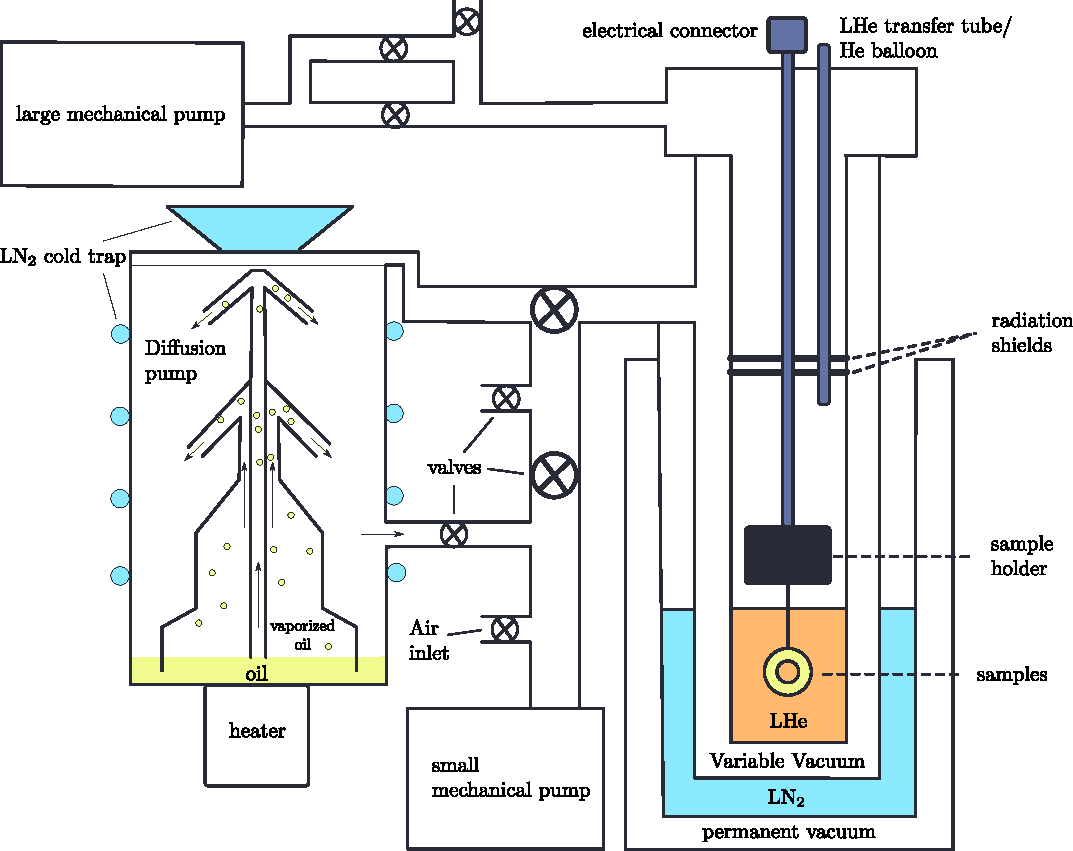
\includegraphics[width = 0.48\textwidth]{apparatus.pdf}
    \caption{Apparatus for Low Temperature Experiments.}
    \label{fig:apparatus}
    \end{center}
\end{figure}
 
Bringing a sample from room temperature ($\sim 300$ K) to low temperatures down to $\sim 1$ K requires three main cooling stages:
First, the variable vacuum is set to roughly 5-10 Torr
with the aid of the small mechanical pump to provide a good thermal connection between the inner and outer dewar.
The samples were then  cooled by filling the outer dewar with liquid nitrogen. 
%could probably omit this part
Although this stage takes several hours to just cool the sample to $\sim 80$ K,
the cheap and abundant liquid nitrogen reduces the cost of cooling the sample with purely liquid helium, a much more expensive and rare resource.

After the sample has reached an equilibrium temperature in the LN$_2$ bath, the variable vacuum pressure must be decreased
to $\sim 10^{-4}$ Torr to close the thermal connection between the inner and outer dewar prior to cooling the sample with liquid helium.
This high vacuum must be attained using the diffusion pump which boils a special oil until it vaporizes and jettisons through a central column.
As the vapor exits the column, the liquid nitrogen cold trap surrounding the walls of the pump quickly condenses the vapor back into a liquid which falls back down in the the
reservoir to be reheated and vaporized again. The free molecular flow of the oil vapors create a jet stream which entrain other gas molecules
through the central column and out the bottom of the pump which ultimately leads to the high vacuum for the variable vacuum.
%% talk about heating diffusion pump crap later on

Before the liquid helium is transferred via a pressure differential from the storage dewar to the inner dewar,
the air inlet must be vented to prevent dangerous pressure build up in the inner dewar which could explode the apparatus.
When the liquid helium is transferred, the sample is cooled very quickly to $\sim 4$ K which does not allow the data acquisition software
to precisely measure the temperature changes of the samples.
%didnt we not do this
To find these intermediate temperatures, the sample would be slowly lifted in order to allow for the sample to warm slowly. This step was unfortunately not done because of a lack of liquid Helium.

% To force the sample to cool more slowly,
% we instead force the sample to heat up slowly by lifting the samples out of the liquid helium bath.

To get to $\sim 1$ K, the large mechanical pump can be used to decrease the 
pressure of the inner dewar.
Although Gay-Lussac's law $P \propto T$ might explain this transition, it is 
actually due to the vapor-liquid phase transition mediated at the surface of the liquid; 
% the when we lower the pressure in the dewar more and more helium has to evaporate to keep vapor pressure and external pressure the same. 
when we lower the pressure in the dewar, the vapor pressure decreases, so the high energy helium molecules on the liquid surface  evaporate out of the liquid which carry the heat energy along with it. This evaporation cools the remaining liquid lowering the temperature of the helium liquid and the samples submerged in it. 
Thus the analog pressure gauge used to monitor the pressure of the inner dewar measures the vapor pressure of the liquid helium which can be used to determine the temperature of the samples using lookup tables \cite{White2001-jq}.

Due to data that was inconsistent with the conditions of the experiment, the thermometer had to be recalibrated. The voltage drop across the thermometer probe at room temperature corresponded to a temperature of ~270 K based on \eqref{calibrate}. To correct for this clearly erroneous reading, a scaling factor of 0.9665 was applied to all computed resistances in order to have the resistance computed at room temperature correspond to room temperature.

\subsection{Analysis}
The uncertainty the dimension measurements of each material propagate into the resistivity calculation and are shown in Tables 1 and 2 for wire and film shaped materials, respectively.
\begin{table}[H]
    \begin{center}
    \begin{tabular}{|c|c|c|c|}
    \hline
    Material & $D$ ($\mu$m) & $L$ (cm) & $\delta \rho / \rho$ \\ 
    \hline
    NbTi & 112 $\pm$ 4 & 10.0 $\pm$ 0.4 & 8\% \\
    \hline
    Cu & 165 $\pm$ 10 & 482.0 $\pm$ 0.5 & 10\% \\
    \hline
    \end{tabular}
    \caption{Dimensions (and their associated uncertainty) of wire-shaped material, with $D$ corresponding to the cross-sectional diameter of the material, and $L$ corresponding to length. The associated uncertainty of the resistivity is given as $\delta \rho / \rho$, calculated via use of \eqref{eq:resistivity}. Uncertainty from the computed resistance is neglected.}
    \label{tab:dimension_wire}
    \end{center}
\end{table}

% For the film-shaped materials,

\begin{table}[H]
    \begin{center}
    \begin{tabular}{|c|c|c|c|c|}
    \hline
    Material & $w$ (mm) & $t$ (mm) & $L$ (mm) & $\delta \rho / \rho$ \\ 
       \hline
    Pb & 1.6 $\pm$ 0.2 & 0.12 $\pm$ 0.01 & 17.0 $\pm$ 0.5 & 20\% \\
       \hline
    Dy & 2.7 $\pm$ 0.2 & 0.11 $\pm$ 0.01 & 18.0 $\pm$ 0.8 & 10\% \\
    \hline
    \end{tabular}
    \caption{Dimensions (and their associated uncertainty) of film-shaped material, wit $w$ corresponding to materials width, $t$ corresponding to thickness, and $L$ corresponding to length. The associated uncertainty of the resistivity is given as $\delta \rho / \rho$, calculated via use of \eqref{eq:resistivity}}
    \label{tab:dimension_film}
    \end{center}
\end{table}

All resistivity in this section are given with the understanding that that the uncertainty corresponding to the material listed in Table \ref{tab:dimension_wire} or \ref{tab:dimension_film} applies. The data presented in the following figures will use a subset of the recorded data for temperatures at which data is dense (below 3 K and above 40 K) in order to highlight trends without frequent overlapping.

The resistivity of Pb was determined from the measured voltages and use of (\ref{eq:resistivity}). The resistivity at their corresponding temperatures are shown in Figure \ref{fig:pb_resistivity}:

% pb_resistivity.pdf inserted here
\begin{figure}[ht]
    \begin{center}
    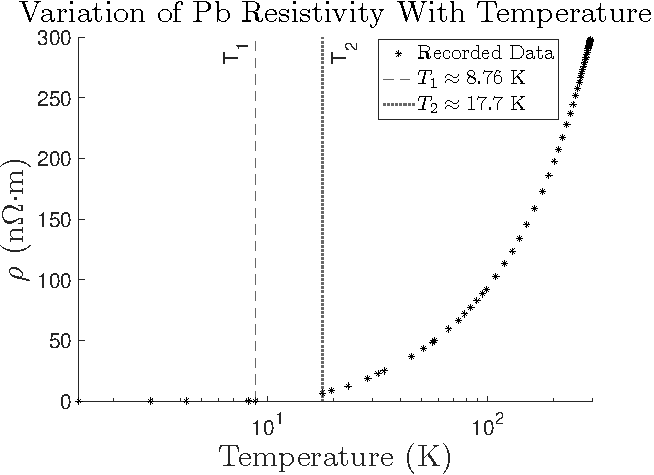
\includegraphics[width = 0.4\textwidth]{pb_final.pdf}
    \caption{Resistivity of lead as a function of temperature. Superconductivity is observed at temperatures measured below $T_1$, and transitions at a temperature between $T_1$ and $T_2$.}
    \label{fig:pb_resistivity}
    \end{center}
\end{figure}
The resistivity of Pb is seen to drop to 0 $\Omega \cdot$m at  $T_1=8.76 \ \text{K}$, with the next nonzero resistivity at $T_2=17.7\ \text{K}$. Due to the lack of data points in this range, it is not possible to make a more precise estimate than $T_c=13.2 \pm 4.5$ K. While the data above $T_2=17.7$ K in Figure \ref{fig:pb_resistivity} follows a linear trend, adherence to this trend cannot be justified within $T_1<T<T_2$, therefore is not used to estimate $T_c.$

Plotting the resistivity of NbTi at different temperatures also showed a transition to superconductivity:
% nbt_resistivity.pdf inserted here
\begin{figure}[H]
    \begin{center}
    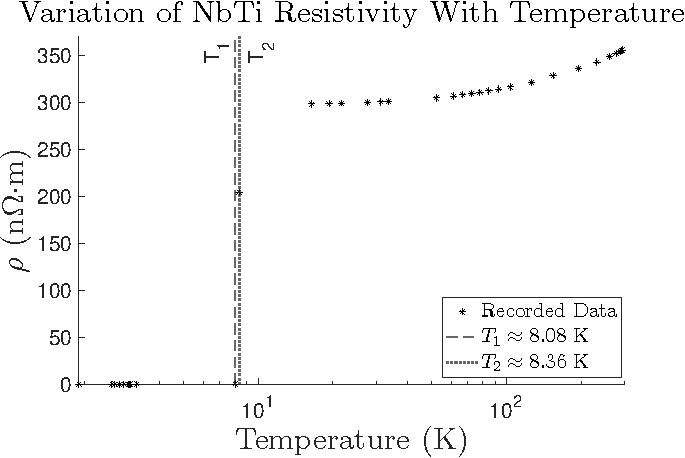
\includegraphics[width = 0.4\textwidth]{nbti_final.pdf}
    \caption{Resistivity of NbTi as a function of temperature. Superconductivity is observed at temperatures measured below $T_1$, and transitions at a temperature between $T_1$ and $T_2$.}
    \label{fig:nbt_resistivity}
    \end{center}
\end{figure}
The first measured temperature at which the resistivity of NbTi drops to 0 $\Omega \cdot$m is seen at $T_1=8.08$ K, with the next nonzero resistivity value recorded at $T_2=8.36$ K. This indicates that $T_c=8.22 \pm 0.14$ K. Similar to Pb, data above $T_2$ is seen to follow a linear trend but is not used to estimate $T_c$ as this trend is seen to break for the recorded value at $T_2$.

Unlike Pb, Figure \ref{fig:nbt_resistivity} implies the resistivity of NbTi experiences an extremely sudden decrease in resistivity near $T_c$, rather than a gradual decrease before reaching 0 $\Omega \cdot$m. Though the data for temperatures just above $T_2$ is sparse, this distinction can still be clearly observed.

\iffalse
The vapor pressure was also determined while the samples were cooling with liquid helium, and compared to data from Cernox's data table \cite{manuel}.
% cernox_vs_vapor.pdf insert
\begin{figure}[H]
    \begin{center}
    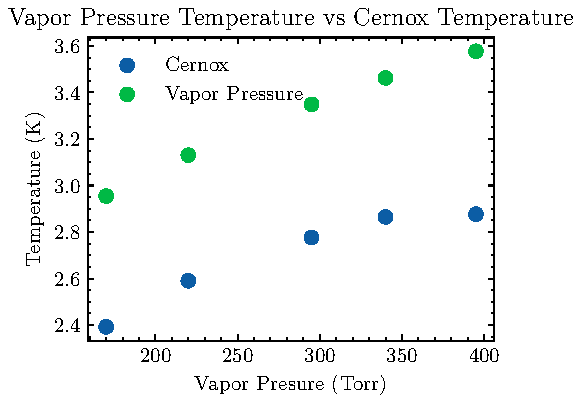
\includegraphics[width = 0.4\textwidth]{cernox_vs_vapor.pdf}
    \caption{Comparison of Cernox and Vapor Pressure Thermometers.}
    \label{fig:cernox_vs_vapor}
    \end{center}
\end{figure}
This graph shows that the recorded data and the vapor pressure follow a somewhat similar trend initially, with the last data point deviating from the values found in their table. The lack of data makes it difficult to determine if this an isolated bad sample, or if other measurements would have resulted in a poor fit with the data. Further, the analog barometer that was used had measurements spaced by 5 Torr, making the collected data somewhat imprecise. The two degree difference between the recorded values and the ones given by Cernox may have been due to the issues in calibration of the thermometer and so the fact the shape is so similar is the most important.
\fi

% resistivity_temp_cu.pdf inserted here
\begin{figure}[ht]
    \begin{center}
    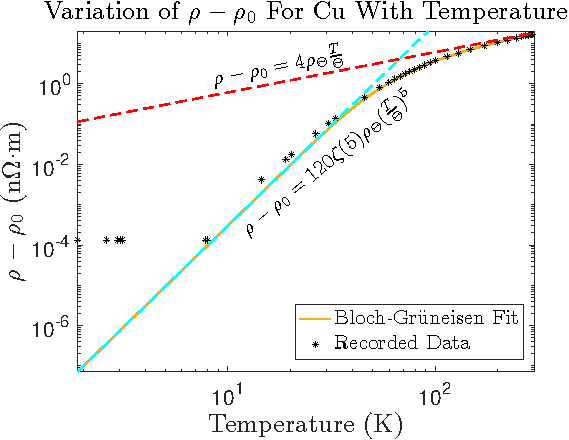
\includegraphics[width = 0.4\textwidth]{cu_final.pdf}
    \caption{Measured resistivity of Copper as a function of temperature compared to a Bloch–Gr\"uneisen fit. The residual resisitivity is removed to highlight the difference in the slope of the data over the range of temperatures. Parameters of the fit are given by $\Theta =316$ K, $\rho_{\Theta}=19.3$ n$\Omega \cdot$m, and $\rho_{0}=0.135$ n$\Omega \cdot$m. At very low temperatures the curves do not match due to noise present in the measured values.}
    \label{fig:resistivity_temp_cu}
    \end{center}
\end{figure}

The Cu sample, unlike the Pb and NbTi samples did not experience a transition to superconductivity:
Measurements below $3.01$ K were seen to result in a resistivity of either $0.135 \ \text{n}\Omega\cdot\text{m}$ or $0.134 \ \text{n}\Omega\cdot\text{m}$, resulting in the sudden divergence of the two curves at lower temperatures. This can likely be attributed to noise or a lack of precision in the recording instruments. 

The recorded data in Figure \ref{fig:resistivity_temp_cu} nearly exactly fit the Bloch–Grüneisen model. The relationship $\rho \propto T^5$ is also clearly seen at lower temperatures, and $\rho \propto T$ is seen to begin near higher temperatures. The reason the trend $\rho \propto T$ is not seen as clearly as the $\rho \propto T^5$ trend can be explained by the recorded temperatures being below $\Theta$, after which this trend is expected to be most accurate.

%Using this fitting, the implied values of the Debeye resistivity, Debeye temperature, resistivity at 0, resistivity at 300 degrees, and RRR, the ratio of resistance at $4.2 \ \text{K}$ and $293\ \text{K}$, are all found. These values were found to be: 
% \iffalse
% \begin{table}[H]
%     \begin{center}
%     \begin{tabular}{|c|c|c|}
%     \hline
%     & Lower Bound & Upper Bound \\
%     \hline
%     $\rho_{\Theta} \ (\Omega \cdot \textrm{m})$ & $1.683 \times 10^{-8}$ & $2.140 \times 10^{-8}$ \\
%     $\Theta$ (K) & $312.3$ & $312.2$ \\
%     $\rho_0  \ (\Omega \cdot \textrm{m})$ & $1.187\times 10^{-10}$ & $1.517 \times 10^{-10}$ \\
%     $\rho_{300}  \ (\Omega \cdot \textrm{m})$ & $1.497\times 10^{-8}$ & $1.9119\times 10^{-8}$ \\
%     RRR & 126.1 & 126.1 \\
%     $R^{2}$ & $1 - 1.486 \times 10^{-5}$ & $1 - 1.824 \times 10^{-4}$ \\
%     \hline
%     \end{tabular}
%     \caption{ Values found fitting data to Bloch Gr\"unseisen}
%     \label{tab:bloch_gruneisen}
%     \end{center}
% \end{table}
% \fi
%The $R^2$ value being nearly exactly 1 attests to how precise the model is able to fit the recorded data. 
%Additionally, the RRR was found. RRR is the ratio of resistance at room temperature (293K) and at liquid helium temperature (4.3K). The RRR is dependent on many factors, one notable one being the purity of the sample, but generally accepted values are between 100-400 \cite{cernRRR}. Our value of 126.1 neatly fits in this range.
Similarly to Cu, Dy was also not seen to exhibit superconductivity.
\begin{figure}[ht]
    \begin{center}
    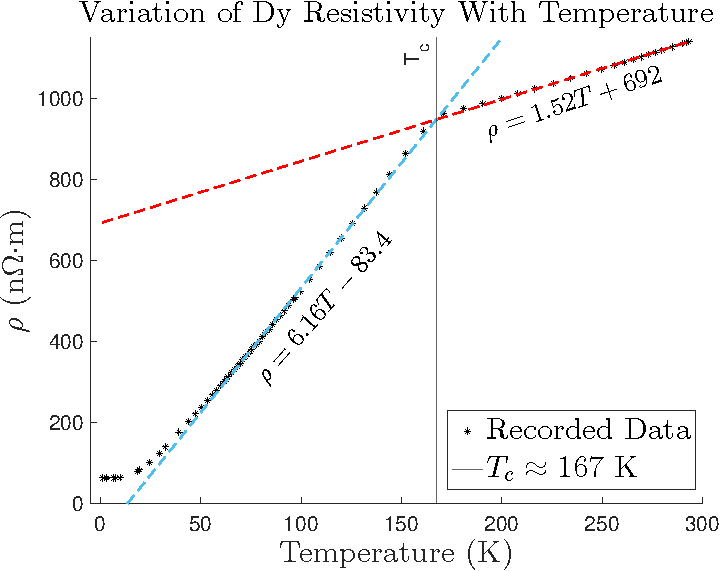
\includegraphics[width = 0.4\textwidth]{dy_final.pdf}
    \caption{Plot of calculated Dy resistivity. The change in slope near the magnetic ordering temperature ($T_c$) is highlighted by the dashed blue and red lines, giving a linear fit using the measurements for lower, and higher temperatures respectively. The units in the equations describing the trend line have units that are implied to match those presented on the axes. Pb's $\rho_0$ is measured to be 62.7 $\Omega \cdot$m.}
    \label{fig:resistivity_temp_dy}
    \end{center}
\end{figure}
Unlike the material previously discussed, Dy is seen to have a drastically different behavior in its resistivity profile at higher temperatures. At around $167$ K, the slope of the trend line followed by the resistivity is seen to suddenly change from around $6.16 \ \frac{\text{n} \Omega \cdot \text{m}}{\text{K}}$ for $T<T_c$ to $1.52 \ \frac{\text{n} \Omega \cdot \text{m}}{\text{K}}$ for $T>T_c$. This break is attributed to a phase change in Dy that occurs around this temperature, in which the material transitions from being  paramagnetic ($T>T_c$) to antiferromagnetic ($T<T_c$).

Due to abundant sampling at lower temperatures and temperatures near room temperature, the RRR can easily be calculated for Dy and Cu. The RRR for NbTi can also be approximated, with the assumption that the flatness seen in the Figure $\ref{fig:nbt_resistivity}$ for measurements at $T>T_2$ holds until the transition to superconductivty begins. Since the resistivity of Pb decreases uniformly to 0 $\Omega \cdot$m above $T_2$ (seen in Figure \ref{fig:pb_resistivity}), a meaningful RRR cannot be assigned.
% \iffalse
% \begin{table}[H]
%     \begin{center}
%     \begin{tabular}{|c|c|c|c|}
%     \hline
%     Material & $\rho_{0}$ (\text{n} \Omega \cdot \text{m})& $\rho_{293}$ $(\text{n} \Omega \cdot \text{m})$ & RRR  \\ 
%     NbTi & 298 & 356 & $1.19 \pm 0.14$ \\
%     Cu & 0.135 & 17.0 & 126 \\
%     Dy & 62.7 & $1.13 \times 10^{3}$ & 18.8 \\
%     \hline
%     \end{tabular}
%     \caption{Dimensions (and their associated uncertainty) of film-shaped material. The associated uncertainty of the resistivity is given as $\frac{\delta \rho}{\rho}$, calculated via use of \eqref{eq:resistivity}}
%     \label{tab:dimension_film}
%     \end{center}
% \end{table}
% \fi
\begin{table}[ht]
    \centering
    \begin{tabular}{|c|c|c|c|}
    \hline
    Material & $\rho_{0}$ $(\text{n} \Omega \cdot \text{m})$ & $\rho_{293}$ $(\text{n} \Omega \cdot \text{m})$ & RRR  \\ 
    \hline
    NbTi & 298 & 356 & $1.19 \pm 0.14$ \\
    \hline
    Cu & 0.135 & 17.0 & $126 \pm 22$ \\
    \hline
    Dy & 62.7 & $1.13 \times 10^{3}$ & $18.8 \pm 3.3$\\
    \hline
    \end{tabular}
    \caption{Computed values of $\rho_{0}$, $\rho_{293}$, and RRR corresponding to the resistivity measured at the lowest achieved temperatures, 293 K, and the residual resistivity ratio, respectively. $\rho_0$ was used in place of the typical $\rho_{4.2}$ due to the fact that $\rho\approx \rho_{0}$ for these samples at all temperatures recorded below $4.2$ K. }
    \label{tab:RRR}
\end{table}

One major source of error in this experiment was the calibration of the thermometer. The initial review of the collected data showed that at room temperature, a voltage of $4.926$ mV---implying a resistance of 49.26 $\Omega$ under a $100$ mA current---corresponding to a temperature of around $278$ K based off the manufacturer calibration settings, which also  predicted a measured resistance of 47.43 $\Omega$ around $293.0$ K. This was corrected for by scaling the measured resistance by a factor of $0.9665$. It is very unlikely that is an accurate way to approach recalibrating the data, and it is likely that the deviations were nonlinear and not possible to accurately model based solely off the data collected in this experiment.

Further, due to a lack of data as a result of equipment malfunction, there is very sparse data in temperature ranges of interest. There is a gap between temperatures of around $3.71$ K and $6.62$ K, as well as $9.74$ K and $18.5$ K (these ranges varied slightly between materials due to a short delay between measurements), which made accurate determination of $T_c$ for Pb impossible. While recorded values for NbTi resistivity luckily allowed for a more precise interval in which $T_c$ could be found, it omits data just before the transition, which would have allowed for a more thorough analysis of the transition to superconductivity.

\section{Conclusion}
In this experiment several  low temperature phenomena were observed in NbTi, Pb, Cu, and Dy. 
% Notably, the transition of NbTi and Pb to superconductivity were clearly observed, the resistivity of Cu was seen to transition from being proportional to $T^5$ to a linear temperature dependence, and a magnetic ordering phase transition in Dy was clearly observed.
Although some values (such as the transition temperature of Pb) were not able to be computed very accurately due to experimental mishaps, the recorded data shows clear transitions of NbTi and Pb to superconductivity, the transition of the resistivity of Cu from $\propto T^5$ to $\propto T$, and a clear phase transition of Dy corresponding to magnetic ordering.

The measured transition temperatures for NbTi and Pb differ slightly from recorded values. NbTi is known to have a transition temperature of $\approx 9.2$ K, differing from the range of $T_c=8.22 \pm 0.14$ K found in this experiment \cite{1062311}.
% [https://www.nature.com/articles/s41598-019-50549-7]
Pb is known to have a transition temperature of $\approx 7.18$ K, which differs from the range $T_c=13.2 \pm 4.5$ K found in this experiment \cite{PhysRev.109.1094}. These deviations are most likely attributed to the improper calibration of the thermometer, as previously discussed.

Likely due to similar issues responsible for the deviation of $T_c$ measured in this experiment from standard values, the magnetic ordering temperature of Dy, found to be $167$ K, is slightly different than the known transition temperature of $179$ K \cite{Wilkinson1961-mk}.
% ^^  
%[https://dr.lib.iastate.edu/server/api/core/bitstreams/59653dc3-610d-471c-a3e0-398827314e74/content]
Neutral Dy also has a recorded $\rho_{0}$ of 24 n$\Omega$m, which differs significantly from the $\rho_0=62.7\pm 6.3$ measured in this experiment. However, another reference lists the RRR of Dy as 17.5 \cite{Sokolenko2024-ls}, falling within the measured RRR of $18.8 \pm 3.3$ in this experiment.

The material properties of copper vary greatly, particularly with the purity of the sample. One study found that different samples of copper can have RRR's ranging from 176 to 1018 \cite{Vorobieva2001-vh}.
\citeauthor*{calatroni2020materialspropertiesthermal} \cite{calatroni2020materialspropertiesthermal} also mentions that some Cu samples can have RRR's of $~100$, some of which are present in Apollonio et al. \cite{cernRRR}. The Debye temperature can also be computed based on the speed of sound, $c_s$, in Cu, which gives a value of $\approx 343$ K \cite{Kittle}. This is slightly different than the computed value of $\Theta=316$ K.

% Despite the deviations between the measurements made in this experiment and measurements from other experiments, as previously mentioned, 
Despite the differences of the measurements made in this experiment in comparison to data from scientific literature, the resistivity profiles of most solids are known to greatly depend on material characteristics such as sample purity, which can vary greatly sample to sample. Therefore, one cannot expect perfect alignment of all of these quantities between different samples. In addition, the the measurements in this experiment were on the same order of magnitude as the values in the literature which makes it reasonable to assume systematic error accounted for a large part of the deviation observed. 

Clearly, the lack of properly calibrated temperature measurements is detrimental to an experiment of this nature. While the values obtained were surprisingly close to the values from the stated references, future renditions of the experiment would greatly benefit from thorough recalibration of the thermometer. Without confidence in the temperature measurements, it is impossible to verify the accuracy of the phase transition temperatures (for both superconductivity and magnetic ordering) for NbTi, Pb, and Dy (as well as the Debye temperature from fitting to the recorded Cu data).

Further, future experiments would also greatly benefit from collection of more data at low temperatures. This would highlight the transitions to superconductivity (especially for NbTi, due to the sparsity of data collected after $T_2$ seen in Figure \ref{fig:nbt_resistivity}).
In order collect more data points to better view the phase transition and estimate the transition temperature, future experiments can lift the samples above the liquid helium bath to slowly warm the samples from $\sim 4$ K until the superconductors reach temperatures near their $T_c$. This would give much more data near temperatures that could not be measured and highlight the nature of the transitions, allowing for a more detailed discussion of some of the phenomena studied in this experiment.
% While this data was intended to be collected, equipment failure prevented this.
%This data would greatly help highlight the behavior of the materials being studied during phase transitions, and allow for a more detailed discussion of the phenomena studied in this experiment.


%the and the different transitions between type I and type II superconductors was not seen. However, the characteristic near zero resistance and super conductance were observed.
%In copper, the residual resistivity at low temperatures from the phonon effects was measured. The collected Cu data showed the characteristic $T^{5}$ scaling of $\rho(T)$ at low temperatures, and $T$ scaling at higher temperatures.

%Using the Bloch-Gr\"uneisen formula, measurements of copper yielded a Debeye temperature of $\Theta_{\text{Cu}}=312.15\pm 0.05 \text{K}$. Copper is estimated to have a Debeye temperature of $\Theta_{\text{Cu}}=343\text{K}$ \cite{Kittle}. While this results in a relative error of $ \approx 8.999\%$ , it is within the same order of magnitude, and the deviation is likely due in part to an improperly calibrated system.

%The RRR values of a given material is known to vary greatly depending on  factors such as the purity of the material. Measurements of the RRR of copper samples typically range from 100-400, which the measured value of 126.1  falls in.\cite{cernRRR}


%Though the measurements collected fit the expected trends, systematic error makes the results difficult to verify exactly. Due to the deviation of the measured thermometer probe resistance from the provided calibration sheet, it is impossible to calculate an accurate temperature. However, recalibration efforts using known values like the room temperature being 293K and the temperature of liquid Helium, the resistance could be fitting to a more closely to the actual temperature. Using this the values were closer to what was expected but the error could not be entirely removed for sections without known temperatures.

% \nocite{PhysRev.21.483} % to add to bibliography without citing
% \nocite{ZimanEP}
\bibliography{myrefs} % myrefs.bib is the bibliography file

\end{document}